\documentclass[a4paper,11pt]{article}

%%%%%%%%%%%%%%%%%%%%%%%%%%%%%%%%%%%%%%%%%%%%%%%%%%%%%%%%%%%%%%%%%%%%%%%%%
\pagestyle{plain}                                                      %%
%%%%%%%%%% EXACT 1in MARGINS %%%%%%%                                   %%
\setlength{\textwidth}{6.6in}     %%                                   %%
\setlength{\oddsidemargin}{-0.06in}   %% (It is recommended that you       %%
\setlength{\evensidemargin}{-0.06in}  %%  not change these parameters,     %%
\setlength{\textheight}{9.1in}    %%  at the risk of having your       %%
\setlength{\topmargin}{0in}       %%  proposal dismissed on the basis  %%
\setlength{\headheight}{-0.1in}      %%  of incorrect formatting!!!)      %%
\setlength{\headsep}{0in}         %%                                   %%
%\setlength{\footskip}{.5in}       %%                                   %%
%%%%%%%%%%%%%%%%%%%%%%%%%%%%%%%%%%%%       
%%%%%%%%%%%%%%%%%%%%%%%%%%%%%%%%%%%%%%%%%%%%%%%%%%%%%%%%%%%%%%%%%%%%%%%%%
 \linespread{1.3}
\usepackage[dvips]{graphicx}
\usepackage{amsmath,bm}
\usepackage{amssymb}
\usepackage{psfrag}
\usepackage{hyperref}
\usepackage{color}
%\usepackage{subfigure}
\usepackage{bigfoot}
\usepackage{framed}
\usepackage{subcaption}
\usepackage{graphicx}

\usepackage[normalem]{ulem}


\newcommand{\bs}{\boldsymbol}
\def\RR{ \mathbb R}
\newcommand{\refeq}[1]{Equation \eqref{#1}}
\def\bl{ \mathbf \lambda}
\def\ba{ \beta}
%%%%%%%%%%%%%%%%%%%%%%%%%%%%%%%%%%%%%
\newcommand{\boxeq}[1]{%
  \[\fbox{%
      \addtolength{\linewidth}{-2\fboxsep}%
      \addtolength{\linewidth}{-2\fboxrule}%
      \begin{minipage}{\linewidth}%
      \begin{equation}#1\end{equation}%
      \end{minipage}%
    }\]%
}
%%%%%%%%%%%%%%%%%%%%%%%%%%%%%%%%%%%%%%%%%%%%%%%%%%%%%%%
\newcommand{\ee}{\end{equation}}
\newcommand{\be}{\begin{equation}}
\newcommand{\ec}{\end{center}}
\newcommand{\bc}{\begin{center}}
\newcommand{\eea}{\end{eqnarray}}
\newcommand{\bea}{\begin{eqnarray}}
\newcommand{\bd}{\begin{description}}
\newcommand{\ed}{\end{description}}
\newcommand{\bi}{\begin{itemize}}
\newcommand{\ei}{\end{itemize}}
\newcommand{\pa}{\partial}

\newcommand{\bx}{\bs{x}}
\newcommand{\bxi}{\bx^{(i)}}
\newcommand{\bxn}{\bx^{(n)}}

\newcommand{\by}{\bs{y}}
\newcommand{\byn}{\by^{(n)}}

\newcommand{\br}{\bs{r}} 
\newcommand{\brn}{\bs{r}^{(n)}} 

\newcommand{\bz}{\bs{z}}

	\newcommand{\pt}{p^{trans}}



\newcommand{\bxx}{\bs{X}}
\newcommand{\bxb}{\bar{\bs{X}}}
\newcommand{\byy}{\bs{Y}}

\newcommand{\bt}{\bs{\theta}}
\newcommand{\btt}{\bs{\Theta}}


\newcommand{\bp}{\bs{\phi}}

\newcommand{\beps}{\bs{\epsilon}}
\newcommand{\qe}{q_{\epsilon}(\bs{\epsilon})}

\newcommand{\bax}{\bs{A}_x}
\newcommand{\bbx}{\bs{b}_x}
\newcommand{\bvx}{\bs{V}_x}
\newcommand{\bcx}{\bs{C}_x}
\newcommand{\bdx}{\bs{D}_x}
\newcommand{\E}{\mathbb{E}}



\newcommand{\psk}[1]{{\color{red} PSK: #1}}


\title{Hydration Model Calibration \& Optimization}
\author{Atul Agrawal}
%\date{\today}

\begin{document}

\maketitle




Notation:
\bi
\item $\bx$: concrete mix parameters (also optimization variables ultimately)
\item $\bs{b}$: hydration model input parameters
\item $\by_c$ or $\by_c(\bs{b})$ : hydration model output(s) relevant for calibration
\item $\by_o$ or $\by_o(\bs{b})$ : hydration model  output(s) relevant for optimization (e.g. KPIs)
\ei
Suppose $N$ data-pairs $\mathcal{D}_N$  are available which consist of $\mathcal{D}_N=\{ \hat{\bx}^{(i)},  \hat{\by}_c^{(i)}\}_{i=1}^N$. We would like to use those to infer the corresponding $\bs{b}^{(i)}$ but more importantly the relation between $\bx$ and $\bs{b}$  which would be of relevance for downstream, optimization tasks.

\section{Calibration}
We postulate a probabilistic relation between $\bx$ and $\bs{b}$ in the form of a density $p(\bs{b}| \bx, ~\varphi)$ where $\varphi$ are associated parameters, e.g.:
\be
p(\bs{b}| \bx, ~\varphi)=\mathcal{N}(\bs{b}| ~\bs{f}_{\varphi} (\bx), \bs{S}_{\varphi}(\bx))
\ee
Let also $p(\hat{\by}_c^{(i)} | \bs{y}_c(\bs{b}^{(i)}))$ the likelihood of each observation $i$. Then:
\be
\begin{array}{ll}
 p(\bs{b}^{(1:N)}, \varphi | \mathcal{D}_N) & \propto p( \hat{\by}_c^{(1:N)} | \bs{b}^{(1:N)})~p( \bs{b}^{(1:N)} | \hat{\bx}^{(1:N)}, \varphi) \\
 & = \prod_{i=1}^N p(\hat{\by}_c^{(i)} | \bs{y}_c(\bs{b}^{(i)}) )~p(\bs{b}^{(i)} | \hat{\bx}^{(i)} , ~\varphi)
\end{array}
\ee

Hence $\bs{b}^{(i)}$ (i.e. the latent model inputs for each concrete mix $i$) and  $\varphi$ would need to be inferred simultaneously. 
Most likely, point estimates for $\varphi$, say $\varphi^*$, would be sufficient at least as the first step.


\section{Optimization (without constraints)} \label{sec:optimisation_wo_constraints}

We define an objective function $o(\by_o)$ with respect to some output(s) of the hydration model. Since the latter depend implicitly on $\bx$ (through $\bs{b}$), we wish to find the value of $\bx$ that e.g. maximizes this objective. Since the relation between $\bx$ and $\bs{b}$ is non-deterministic i.e. for a single $\bx$ there could be multiple $\bs{b}$ and therefore multiple $\by_o(\bs{b})$, we consider the expected value of the objective, say:
\be \label{eq:opt_1}
V(\bx)= \int o(\by_o(\bs{b})) ~p(\bs{b} | \bx, \varphi^*) ~d\bs{b}
\ee
We denote with  $\varphi^*$ the point-estimates of $\varphi$ found in the Calibration step above.
For example if $o(\by_o)$ is the indicator function of some event relating to $\by_o$, then by maximizing  $V(\bx)$, we maximize the probability of this event.

To carry out the optimization, derivatives of ${V}(\bx)$ would be needed. These can be expressed as:
\be
\begin{array}{ll}
\frac{\pa V}{\pa \bx} & = \int o(\by_o(\bs{b})) ~\frac{\pa p(\bs{b} | \bx, \varphi^*) }{\pa \bx}~d\bs{b} \\
& = \int o(\by_o(\bs{b})) ~\frac{\pa ~\log p(\bs{b} | \bx, \varphi^*) }{\pa \bx}~ p(\bs{b} | \bx, \varphi^*) ~d\bs{b} \\
\end{array}
\label{eq:gv1}
\ee
Assuming the derivatives $\frac{\pa \log p(\bs{b} | \bx, \varphi^*) }{\pa \bx}$ can be computed, the integral above can be approximated by Monte Carlo and sampling $\bs{b}^{(m)}$ from  $p(\bs{b} | \bx, \varphi^*)$ i.e. as:
\be\label{eq:opt_3}
\begin{array}{ll}
\frac{\pa V}{\pa \bx} & \approx \frac{1}{M} \sum_{m=1}^M  o(\by_o(\bs{b}^{(m)} )) ~\frac{\pa~ \log  p(\bs{b}^{(m)} | \bx, \varphi^*) }{\pa \bx} \\
\end{array}
\ee 
The Monte Carlo estimates can then be used in a stochastic gradient ascent scheme to identify the optimum $\bx$. Note that \textbf{no derivatives of the hydration model  } would be needed.


If we assume that the density $p(\bs{b} | \bx, \varphi^*)$ is reparametrizable \cite{schulman_gradient_2016} (e.g. Gaussian) and one can write it as a differentiable  transformation (ignoring $\varphi^*$ in order to simplify the notation): 
\be
\bs{b}=\bs{g}_{\bx}(\bs{z})
\ee
where $\bs{z}$ follow a known density, say $p(\bs{z})$, then with a change of variables:
\be
V(\bx)= \int o(\by_o( \bs{g}_{\bx}(\bz ))) ~p(\bs{z}) ~d\bs{z}
\ee
and:
\be
\begin{array}{ll}
\frac{\pa V}{\pa \bx} & = \int \frac{\pa o }{ \pa \by_o } \frac{\pa \by_o }{ \pa \bs{b} } \frac{\pa \bs{g}_{\bx}(\bz) }{ \pa \bx }
 ~p(\bs{z}) ~d\bs{z}
 \\
\end{array}
\ee

The gradient above can be estimated by sampling $\bz^{(m)}$ from $p(\bz)$ and evaluating the other terms, i.e. as:
\be
\begin{array}{ll}
\frac{\pa V}{\pa \bx} &  \approx \frac{1}{M} \sum_{m=1}^M \frac{\pa o^{(m)} }{ \pa \by_o } \frac{\pa \by_o^{(m)} }{ \pa \bs{b} } \frac{\pa \bs{g}_{\bx}(\bz^{(m)}) }{ \pa \bx } \\
\end{array}
\ee
where $\bs{b}^{(m)}=\bs{g}_{\bx}(\bz^{(m)})$, $\by_o^{(m)}=\by_o ( \bs{b}^{(m)})$ and $o^{(m)}=o(\by_o^{(m)})$.
While it is anticipated that the variance of these Monte Carlo estimates of the gradient of $V$ will be smaller as compared to \refeq{eq:gv1}, they would require a differentiable ${o}(.)$ (usually feasible) and a differentiable model $\bs{y}_o(\bs{b})$ (i.e. potentially adjoints).

The calibration and optimisation frameworks can also be viewed as probabilistic graphs. For the current configuration, the probabilistic graph is given by Fig. \ref{fig:prob_graphs}. 
With slight notational abuse, same skeletal can be employed for calibration and the optimisation module. There is just a change of observed and unobserved variables. This is a generalised framework for any number of nodes and edges. In theory, if the conditionals are provided, calibration/optimisation can be performed for any level of hierarchy in the graph.

The variables and the relations associated are explained in points below:

\begin{itemize}
    \item The variables associated are explained in the starting of the document. 
    \item The probabilistic relation $p(\bs{b} | \bx; \varphi)$ between $\bm b$ and $\bm x$ can be given by a parametrised Normal distribution (example usecase in section \ref{calibration_section}). It can be a Gaussian process, Bayesian Neural Nets or anything similar also.
    \item In the example usecase in section \ref{calibration_section}), the probabilistic relation between the latent $\bm b $ and the observed $\bm \hat{y}$ is given by a Normal distribution which needs a deterministic solver given by $\bm y(\bm b)$. In the example, its just a simple linear function, it can be any black box physics based solver.
    \item Similarly, to elaborate the optimisation graph more, consider section \ref{opt_section}. Here $\bm x$ is the optimisation variable with $\bm \varphi^*$ known from the calibration. The probabilistic relation between  $\bm b $ and the $\bm \hat{\bm y}$ is given by the objective function. It is the Mean Square error in the example ($o(\bm{y}_0(\bm{b})) = || \bm{\hat{y}_0} - \bm{y}_0(\bm{b}) ||_2$). Or the variable $\bm \hat{y}$ can also represent the target domain $\mathcal{Y}$ if $o(\bm y_o(\bm b))$ is given by some indicator function $\mathbb{I}_{\mathcal{Y}}(\bm y_o)$. For example, for Hooke's law, one can have objective such as given certain strain, maximise the probability that the stress (given by $\bm y_o(\bm b)$ ) is greater than $\hat{\bm y}_o$ 
    
\end{itemize}

\begin{figure}[!htpb]
\centering
\begin{subfigure}{0.4\textwidth}
    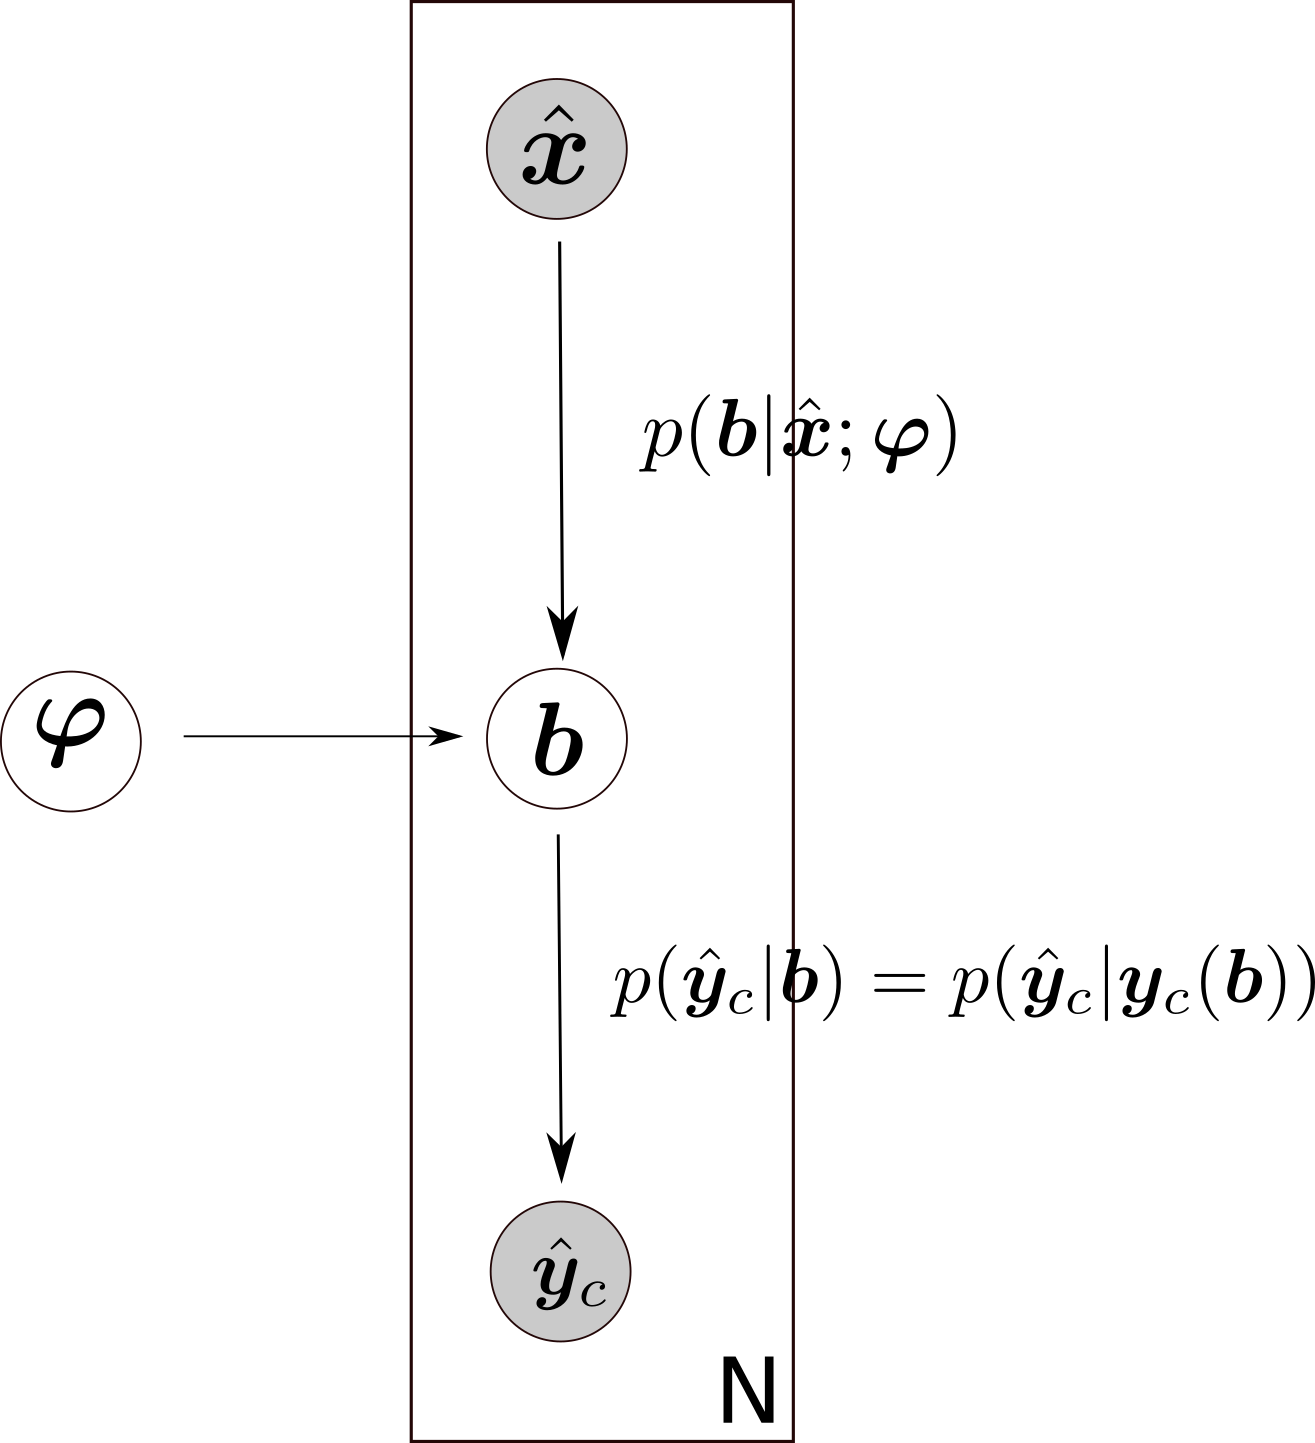
\includegraphics[width=\textwidth]{fig/Calibration_graph.png}
    \caption{Probabilistic graph for the calibration module}
    \label{fig:cal_graph}
\end{subfigure}
\hfill
\begin{subfigure}{0.4\textwidth}
    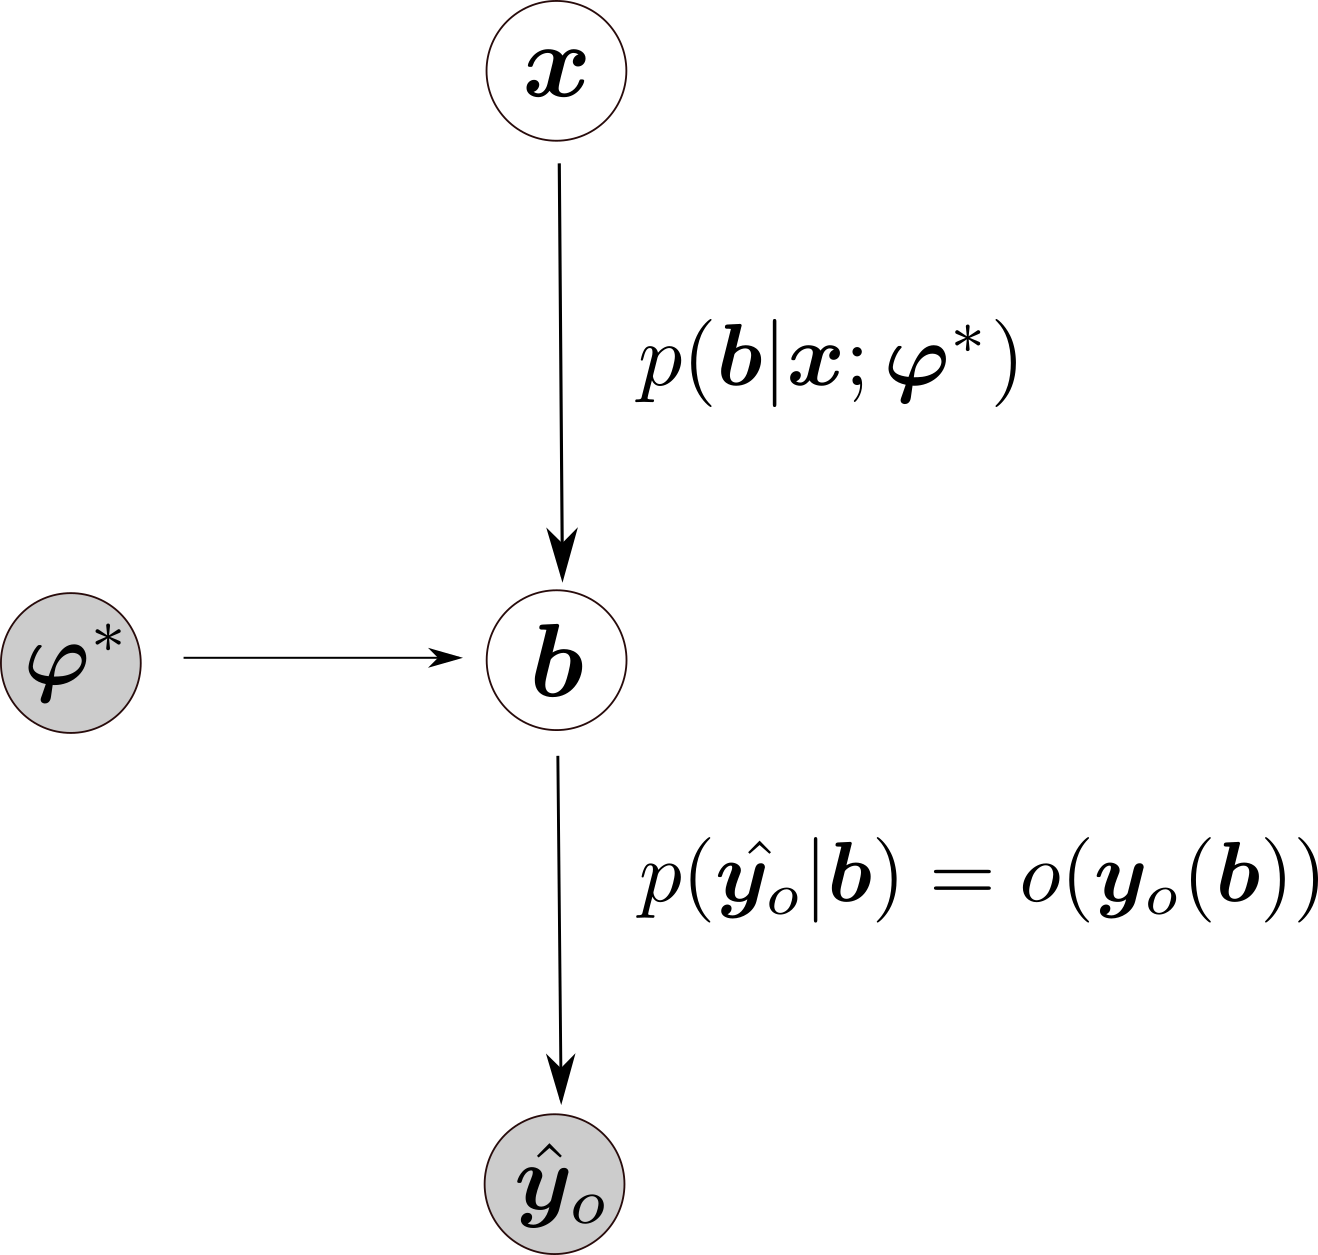
\includegraphics[width=\textwidth]{fig/Optimisation_graph.png}
    \caption{Probabilistic graph for the optimisation module}
    \label{fig:opt_graph}
\end{subfigure}
\caption{\emph{The probabilistic graphs} : Hollow circle - latent/unobserved variables, grey circle-observed/known variables, $\longrightarrow$ - conditionals with data driven/physics based models. Note that optimisation can also be interpreted as a inference task, hence can be cast on the same skeletal. }
\label{fig:prob_graphs}
\end{figure}



% ------------------------------------------------
\clearpage
\subsection*{Additional Notes on Calibration}
To determine $\varphi^*$, we would need to perform the following:
\begin{align*}
    \varphi^* = \arg \max_{\varphi} \log p(\mathcal{D}_N|\varphi)
\end{align*}
Since this involves computations of deterministic values of the parameter $\varphi$, \textit{Expectation-Maximisation} scheme can be employed. A lower bound to the log-evidence can be found out by Jensen's inequality. It says the optimal density which makes the lower bound tight is the posterior $p(\bs{b}^{(1:N)} | \mathcal{D}_N, \varphi)$. The marginal log-likelihood/evidence is given by:

\begin{align}
    \log p(\mathcal{D}_N|\varphi) &= \sum_{i=1}^N\log \int p(\bm {b}^{(i)},\mathcal{D}_N| \varphi)d\bm {b}^{(i)}\\
    &= \sum_{i=1}^N \log \int p(\mathcal{D}_N | \bm {b}^{(i)}) p(\bm b^{(i)}|\bm x^{(i)};\varphi) d\bm b^{(i)}\\
    &\geq \sum_{i=1}^N \langle \log \frac{ p(\mathcal{D}_N | \bm b^{(i)}) p(\bm b^{(i)}|\bm x^{(i)};\varphi)}{q_i(\bm b^{(i)})} \rangle_{q_i(\bm b^{(i)})}=\mathcal{F}(q_{1:N},\varphi)
\end{align}

\begin{itemize}
    \item E-step: Fix $\varphi$ and update $q_i(\bs{b}^{(i)})$. The optimal $q(\bs{b})$ is the conditional posterior i.e.   
    \begin{align}
        q_i^{opt}(\bm b^{(i)}) = p(\bm b^{(i)}|\mathcal{D}_N, \varphi) \propto p(\hat{\by}_c^{(i)} | \bm b^{(i)}) p(\bm b^{(i)} | \bm x^{(i)}, \varphi)
    \end{align}
    This ensures that the inequality is tight. Suppose one obtains $M$  samples $\bs{b}^{(i)}_{1:M}$ of EACH OF THESE (conditional) posteriors using MCMC\footnote{Store the last sample from the previous E-step and use it as starting point of the MCMC in the next E-step}. Note, this step can be parallelized. 
    \item M-step: Given $\{q_i(\bs{b}^{(i)})\}_{i=1}^N$ compute derivatives of the ELBO w.r.t $\varphi$ in order to update them. Note that:
    \be
    \frac{\pa \mathcal{F}}{\pa \varphi} = \sum_{i=1}^N \left< \frac{\pa \log p(\bm b^{(i)}|\bm x^{(i)};\varphi)}{\pa \varphi}} \right>_{q_i}
    \ee
    If the latter expectation is approximated with the MCMC samples above, then:
    \be
    \frac{\pa \mathcal{F}}{\pa \varphi}  \approx \sum_{i=1}^N \frac{1}{M} \sum_{m=1}^M  \frac{\pa \log p(\bm{b}_m^{(i)}|\bm x^{(i)};\varphi)}{\pa \varphi} }
    \ee
    and a stochastic gradient ascent algorithm would need to be employed.
    Note that one does not need to update all the $\bs{b}^{(i)}$-posteriors. It would suffice that e.g. only one is updated and the rest are kept the same (see R.Neal "A view of EM ...") i.e. new samples $\bm{b}_m^{(i)}$ are drawn from one or more $q_i^{opt}$ while for the rest, the samples of the previous posteriors (even though $\varphi$ has changed) are re-used in the estimate above. Of course this would increase the number of EM iterations that would be needed but each iteration would be cheaper.
    It is also possible to use Monte Carlo to approximate the sum over $i$ above. One could randomly select an index $j$, update only  $q_j^{opt}$, i.e. draw MCMC samples from it and use a Monte Carlo estimate of the gradient as:
     \be
    \frac{\pa \mathcal{F}}{\pa \varphi} \approx N  \frac{1}{M} \sum_{m=1}^M  \frac{\pa \log p(\bm{b}_m^{(j)}|\bm x^{(j)};\varphi)}{\pa \varphi} }
    \ee
    Of course this would increase the noise  in the estimate of the derivative and  probably require more EM iterations  but each iteration would be cheaper.
% Compute the log marginal, and perform optimisation optimisation with the grad given by  (Classical optimisation algo can be used here for eg ADAMS).
%    \begin{align}
%        &\langle \frac{\partial \log p(\mathcal{D}_N|\varphi) }{\partial \varphi} \rangle_ {q(\bm b)}\\
%        or ,&\langle \frac{\partial \log p(\bm b|\bm x;\varphi) }{\partial \varphi} \rangle_ {q(\bm b)}
%    \end{align}
\end{itemize}

\underline{Simplest first steps}
\begin{itemize}
    \item Generate synthetic data $\mathcal{D}_N$
    \begin{itemize}
        \item Prescribe models:
        \bi
        \item $p(\bs{b} | \bx, \varphi)$,
        \item $\by_c(\bs{b})$ 
        \item $p(\hat{\by}_c | \by_c(\bs{b}))$.
        \ei
      \item Select some value  $\varphi$ 
      \item Select $\{\bm{x}^{(i)}\}_{i=1}^N$
        \item Draw  $\bm{b}^{(i)} \sim  p(\bs{b}^{(i)} | \bx, \varphi),~i=1,\ldots N$
        \item compute $\by_c(\bs{b}^{(i)})$ 
        \item Draw $\hat{\by}_c^{(i)} \sim   p(\hat{\by}_c^{(i)} | \by_c(\bs{b}^{(i)})),~i=1,\ldots N$
        % . Here, $f$ can be linear, polynomial/ NN etc.
      %  \item $\hat{\bm y}^{(i)} = y_c(\bm{b}^{(i)}) + \text{noise}$
      \item Then $\mathcal{D}_N=\{ \bm{x}^{(i)}, \hat{\by}_c^{(i)} \}_{i=1}^N$
    \end{itemize}
    \item Use $\mathcal{D}_N$ to infer $\bs{b}$ and find $\varphi$. Compare with the known values. As $N\to \infty$ you should recover ground truth.
    \item If the forward solver is prohibitively expensive, surrogate it with GP and propagate its uncertainty in the likelihood.
    \item With the learnt $\varphi^*$, perform the predictions/optimisation tasks downstream.
    \item Since there is FEM solver here, I think getting a closed form solution in E step would be difficult, so VI needs to be employed to get an approximate dist.
\end{itemize}

\section{Numerical Experiment}

\subsection{\emph{Calibration}}\label{calibration_section}

% The formulation is tested on a Bohachevsky function\footnote{https://www.sfu.ca/~ssurjano/boha.html}, which has a bowl shape. This function is chosen as a substitute to some expensive FEM model. The inputs to the function are considered to be be latent and parameterised by $\varphi$. The models considered are as follows:

% \begin{itemize}
%     \item $\bm{y}_c(\bm b) = b_1^2 + 2b_2^2 -0.3\cos(3\pi b_1) - 0.4\cos(4 \pi b_2) + 0.7$
%     \item $p(\bs{b} | \bx, \varphi) = \mathcal{N}(\bs{b}| \bm \varphi^T \bm x, \Sigma_p)$
%     \item $p(\hat{\by}_c | \by_c(\bs{b})) = \mathcal{N}(\hat{\by}_c|\bm{y}_c(\bm b),\Sigma_l)$
% \end{itemize}

% For a given $\bm \varphi$ and $\{\bm{x}^{(i)}\}_{i=1}^N$, synthetic data $\mathcal{D}_N$ is generated and the goal is to recover $\{q_{(i)}(\bm b^{(i)})\}_{i=1}^{N}$ and $\bm \varphi$ with the $E-M$ algorithm as described above.

Simple linear function is chosen as a substitute to some expensive FEM model. The inputs $\bm b$ to the function are considered to be be latent and parameterised by $\varphi$. The models considered are as follows:

\begin{itemize}
    \item $\bm{y}_c(\bm b) = \bm A \bm b + \bm B; \quad \bm{y}_c \in \mathbb{R}^{10}, \bm b \in \mathbb{R}^2$ \quad \text{with} $\bm A, \bm B$ being coefficients. 
    \item $p(\bs{b} | \hat{\bm x}; \varphi) = \mathcal{N}(\bs{b}| \bm \varphi \hat{\bm x}, \Sigma_p) \quad \bm x \in \mathbb{R}^2, \bm \varphi \in \mathbb{R}^{2}$
    \item $p(\hat{\by}_c | \by_c(\bs{b})) = \mathcal{N}(\hat{\by}_c|\bm{y}_c(\bm b),\Sigma_l)$
\end{itemize}

For a given $\bm \varphi$ and $\{\hat{\bm x}^{(i)}, \hat{\bm y}_c\}_{i=1}^N$, noisy synthetic data $\mathcal{D}_N$ is generated and the goal is to recover $\{q_{(i)}(\bm b^{(i)})\}_{i=1}^{N}$ and $\bm \varphi$ with the $E-M$ algorithm as described above.

Figure \ref{fig:EM_diagnostics} discusses the results of the numerical experiment performed. The synthetic data was generated with $\bm \varphi$ beings $1's$. For random starting value of $\bm \varphi$ and $\bm b$, it is interesting to note that the parameters $\bm \varphi$ is learnt as per Fig. \ref{fig:para_EM}. The ELBO gradients are given in the Fig. \ref{fig:grad_EM} Probabilistic estimate of the latent $\bm b$ are also inferred (Fig. \ref{fig:q_N_EM}). For all the observed data pairs, the inferred latents envelope the ground truth. Its worth mentioning the following points:

\begin{itemize}
    \item More complex parametric model like a NN. GP etc can be employed for $p(\bs{b} | \bx, \varphi)$.
    \item Currently a simple Random walk MCMC is used. If $\bm{y}_c(\bm b)$ is computationally expensive, then either a cheaper surrogate needs to be used or the solver needs to be differentiable.
    \item Currently, point estimate of the parameter is learnt. If a probabilistic estimate needs to be made, variational inference needs to be performed. (EM is just a special case of VI with direc delta on the parameters)
\end{itemize}


% ---------------

\begin{figure}[!htpb]
\centering
\begin{subfigure}{0.45\textwidth}
    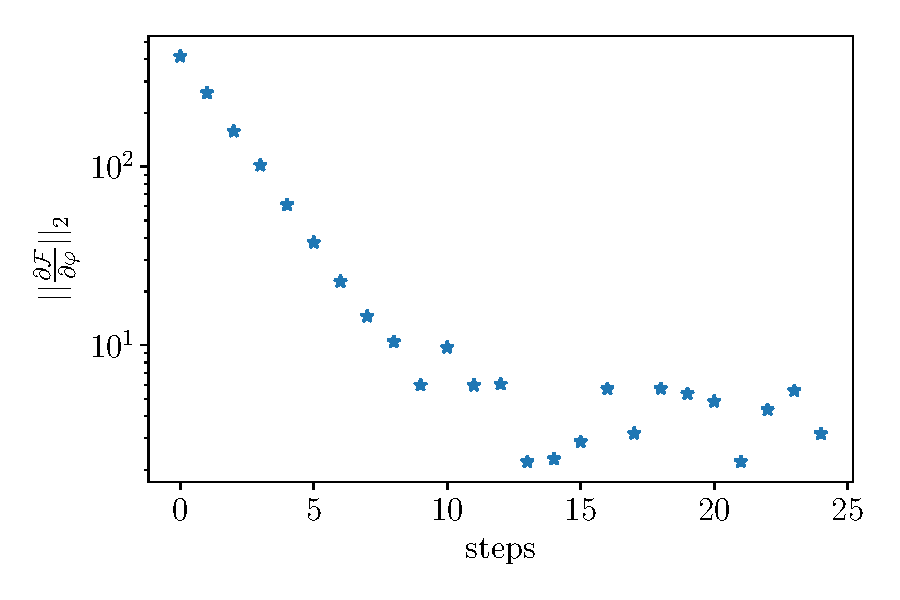
\includegraphics[width=\textwidth]{fig/grad_07_07_2022.pdf}
    \caption{$L_2$ norm of the ELBO gradients}
    \label{fig:grad_EM}
\end{subfigure}
\hfill
\begin{subfigure}{0.45\textwidth}
    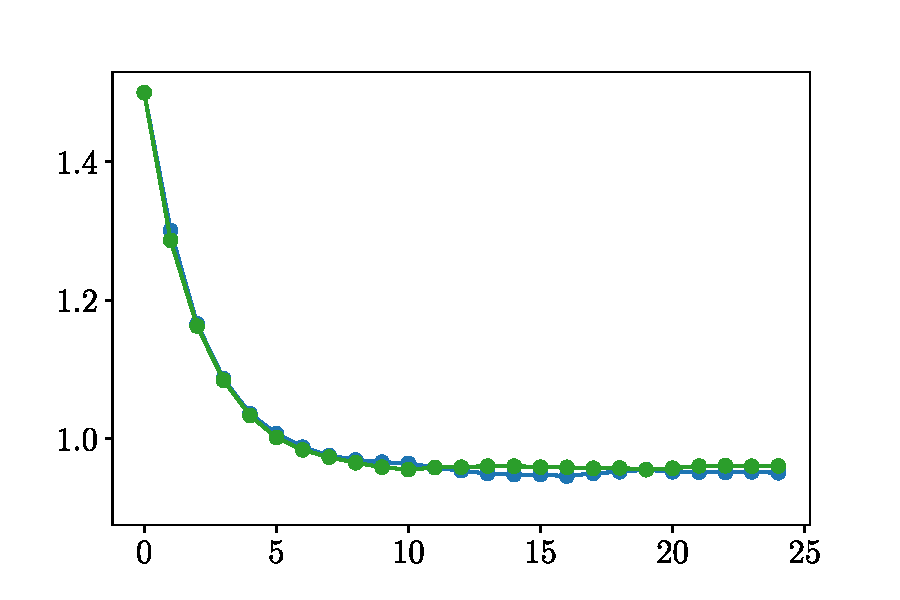
\includegraphics[width=\textwidth]{fig/para_individual_updated.pdf}
    \caption{Evolution of the parameters, Green and blue colors represent $\phi_1$ and $\phi_2$ respectively.}
    \label{fig:para_EM}
\end{subfigure}
\caption{EM step diagnostics}
\label{fig:EM_diagnostics}
\end{figure}

\begin{figure}[!htpb]
    \centering
    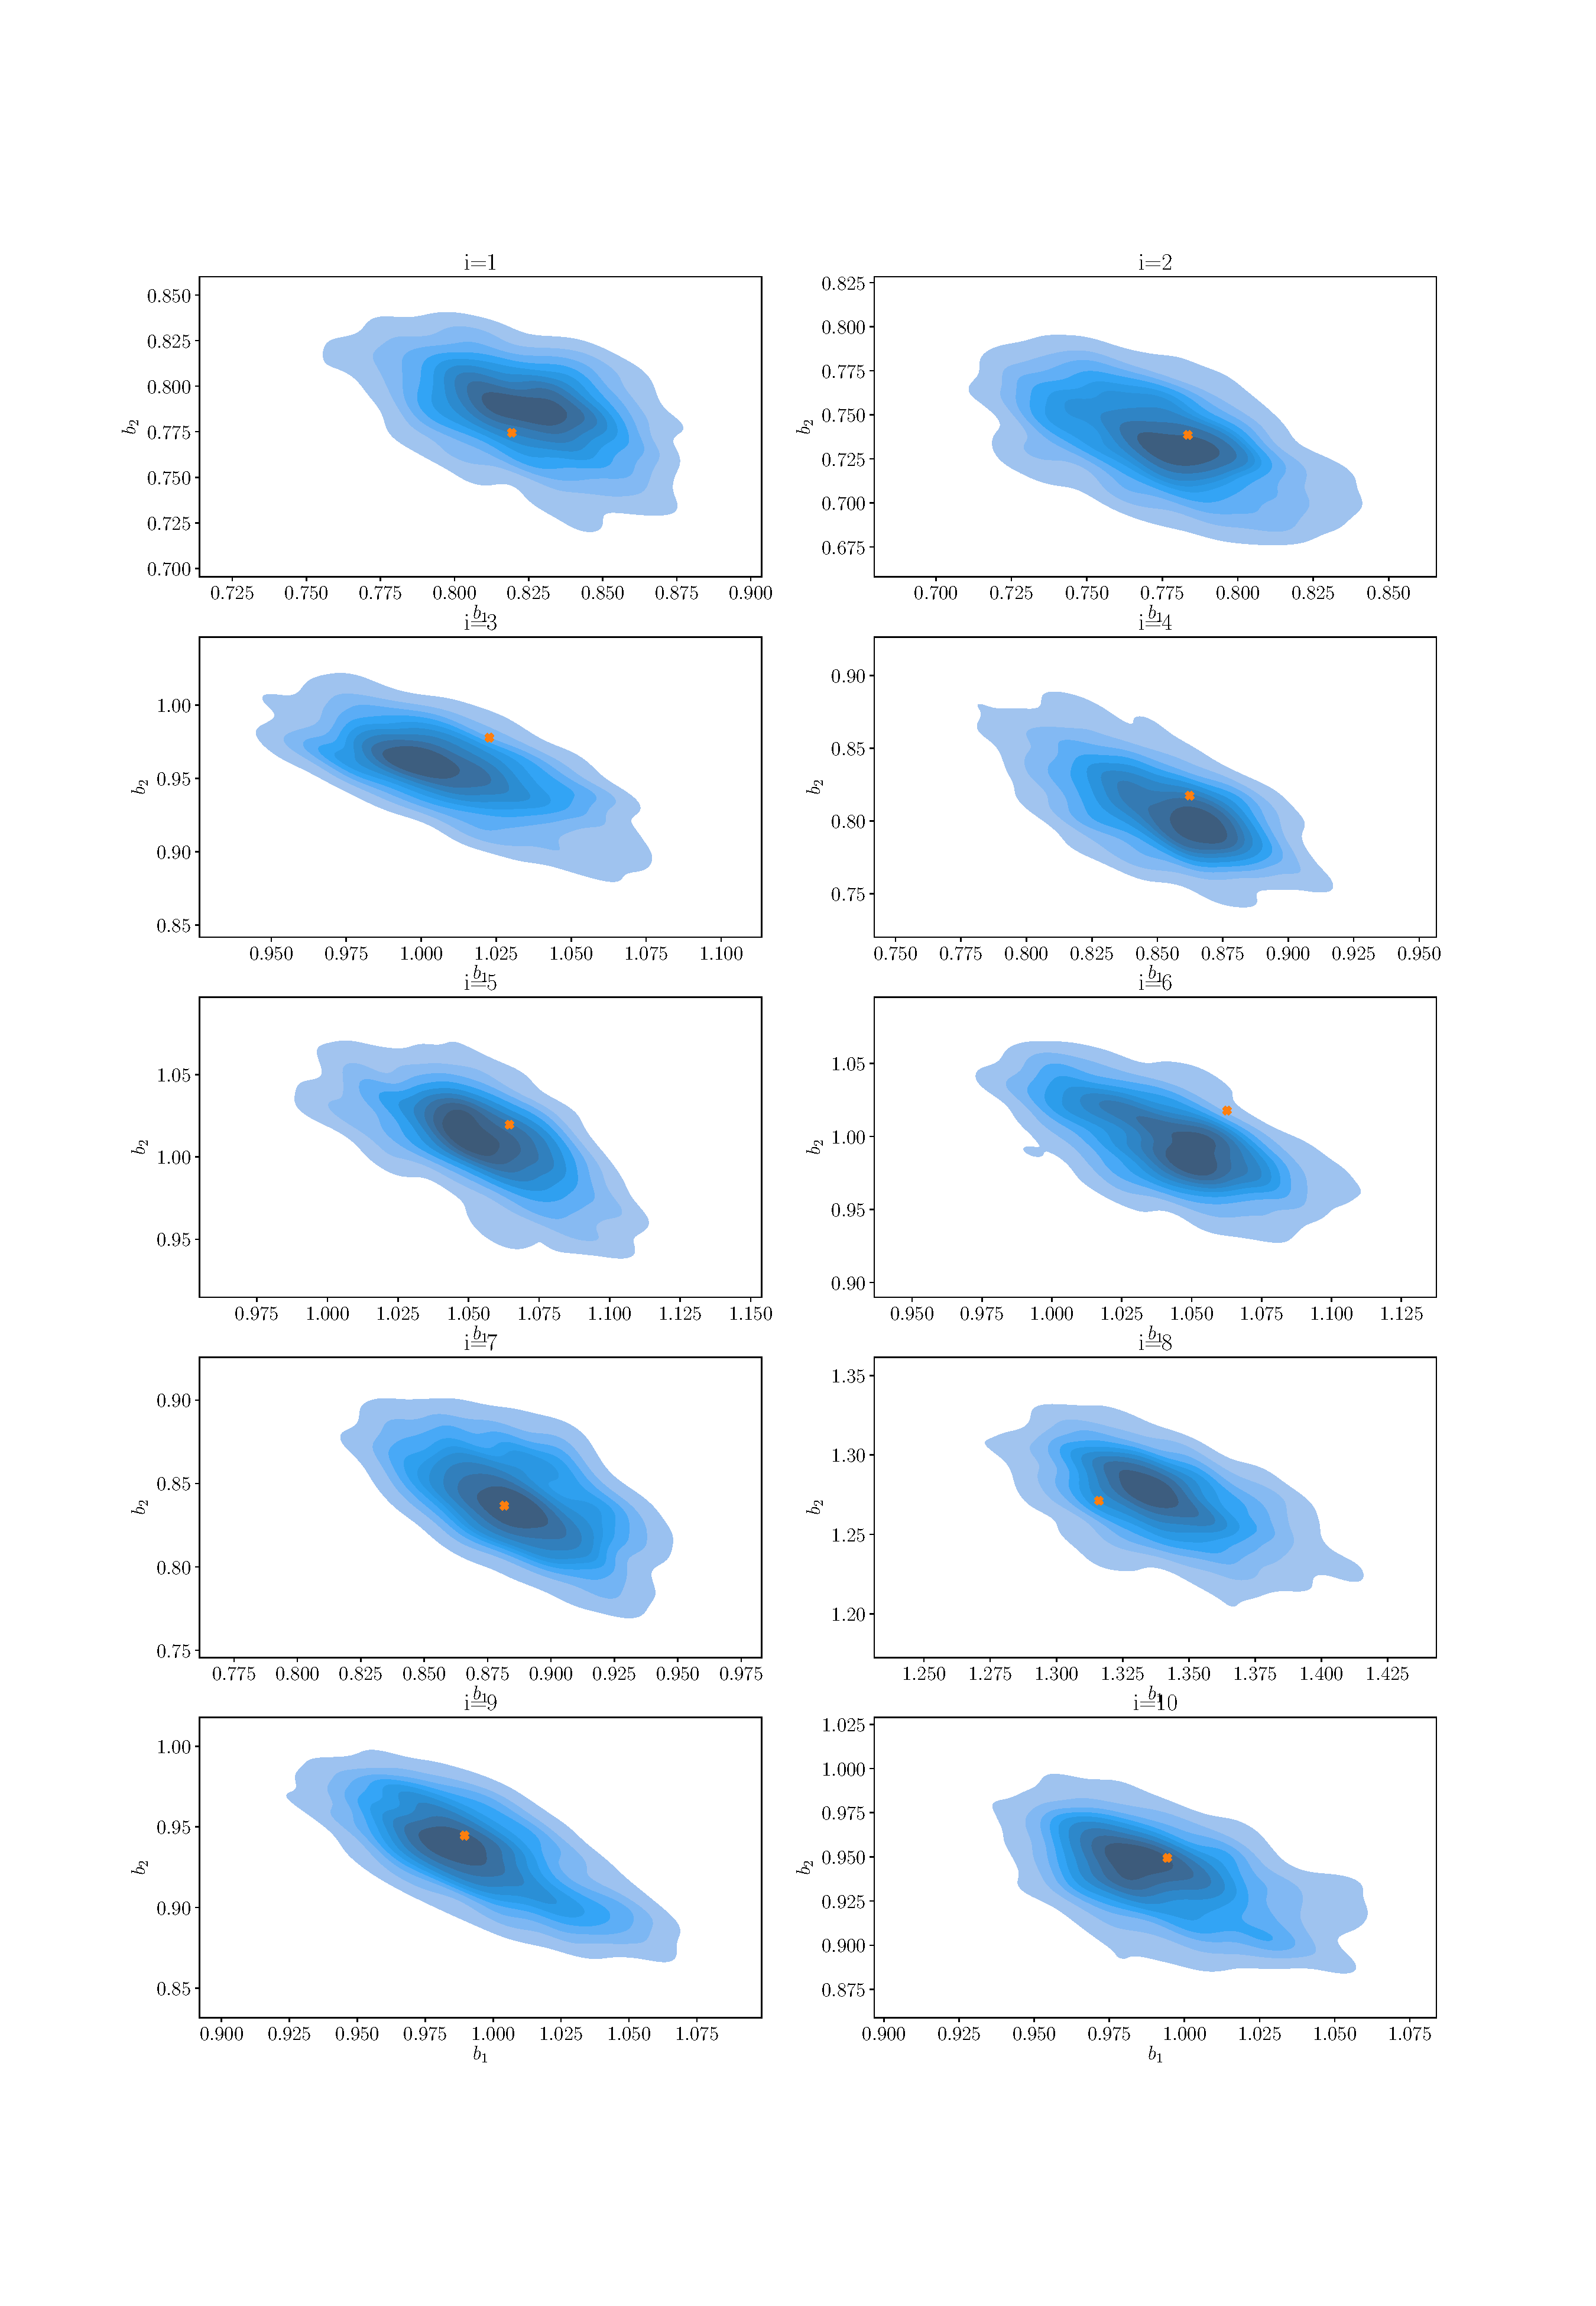
\includegraphics[width=\textwidth]{fig/q_N_Emsteps_01_07_2022.pdf}
    \caption{The latent $\bm b$ samples of the last EM step for N number of observed data. In orange are the "true" values for comparison.}
    \label{fig:q_N_EM}
\end{figure}

\subsection{\emph{Optimisation}}\label{opt_section}

Similar to the numerical experiment performed for the calibration task, the same simple linear model is chosen to demonstrate the capabilities of the optimisation algorithm. Here the parameters $\bm \varphi^*$ is known from calibration and the optimum $\bm x^*$ needs to be identified. The experiment is performed with the following configuration:

\begin{itemize}
    \item $\bm{y}_o(\bm b) = \bm A \bm b + \bm B; \quad \bm{y}_c \in \mathbb{R}^{10}, \bm b \in \mathbb{R}^2$ \quad \text{with} $\bm A, \bm B$ being coefficients. 
    \item $p(\bs{b} | \bx, \varphi^*) = \mathcal{N}(\bs{b}| \bm \varphi^* \bm x, \Sigma_p) \quad \bm x \in \mathbb{R}^2, \bm \varphi^* \in \mathbb{R}^{2}$
    \item Generating synthetic data : Take the $\bm \varphi^*$ value from the calibration step, fix $\bm x$, generate few realisations of $\bm b$ and then compute $\bm{y}_o(\bm b)$ (lets call it $\bm{\hat{y}_0}$)
    \item $o(\bm{y}_0(\bm{b})) = || \bm{\hat{y}_0} - \bm{y}_0(\bm{b}) ||_2 $ with $\bm{\hat{y}_0}$ being synthetically generated observed data.
    \item $\bm x^*  = \arg \min V(\bm x)$ (Eq. \ref{eq:opt_1} - Eq. \ref{eq:opt_3}) is performed using ADAMS (Used hand coded optimiser as grads are approximated by Monte Carlo. )
\end{itemize}

The evolution of the design variable $\bm x$ is given in Fig. \ref{fig:para_opt} and the Monte Carlo estimates of the gradients are given in Fig. \ref{fig:grad_opt}. It is important to note that the optimizer converged to an optimum value (The value was used to generate the observed synthetic data). It is noteworthy that the variance of the estimated gradients controls how the optimizer behaves near the optimum. For a tight variance near the optimum, better Monte Carlo estimates (need more samples $M$) are preferred. However it also amounts to a increased computational cost, which necessitates efficient surrogate to compute the objective.

\begin{figure}[!htpb]
\centering
\begin{subfigure}{0.45\textwidth}
    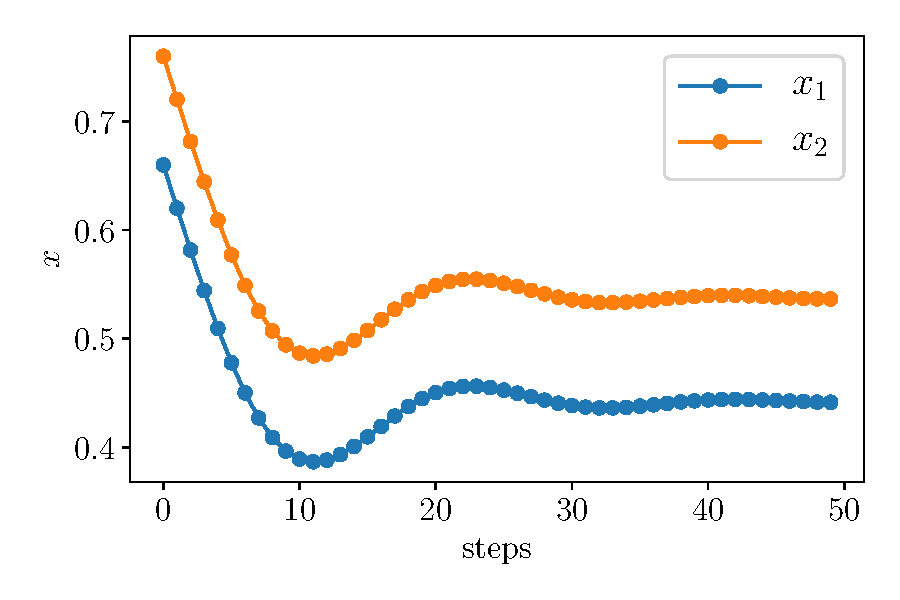
\includegraphics[width=\textwidth]{fig/optimised_x_17_08_2022_15:12.pdf}
    \caption{Evolution of the optimisation variable $x$}
    \label{fig:para_opt}
\end{subfigure}
\hfill
\begin{subfigure}{0.45\textwidth}
    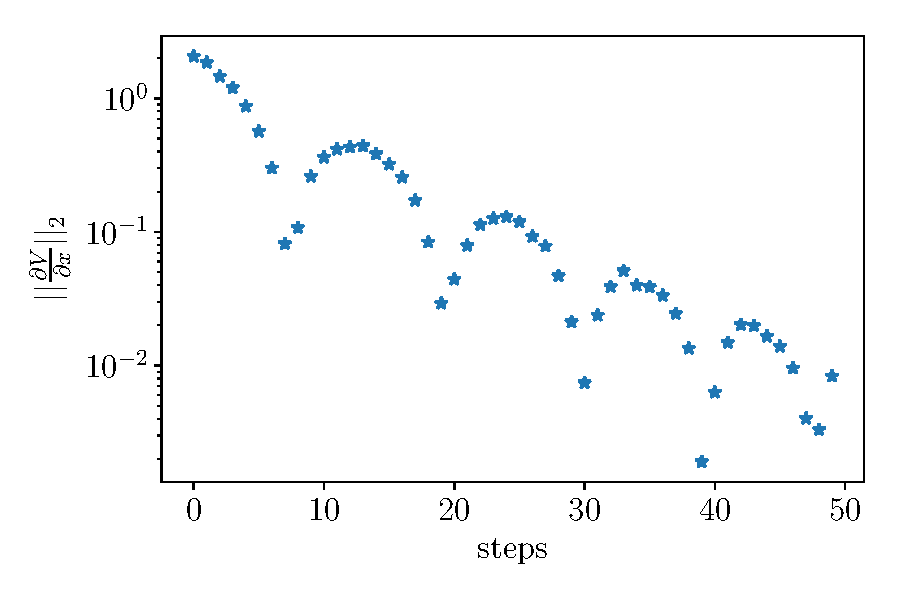
\includegraphics[width=\textwidth]{fig/grad_optimisation_17_08_2022_15:12.pdf}
    \caption{Monte Carlo estimated gradients}
    \label{fig:grad_opt}
\end{subfigure}
\hfill
\caption{Optimisation under uncertainty}
\label{fig:opt_diagnostics}
\end{figure}

\subsection{Calibration and Optimisation of Concrete hydration model}

A finite element based macro scale hydration model for early age concrete is performed \footnote{}. Let the hydration model be given as a function $\bm{y} : \mathbb{R}^4 \rightarrow \mathbb{R}^D$ which maps the latent model parameter of the hydration model given by $\bm b$ to the latent heat of hydration $\bm Q$, for $D$ time steps. The observed data is assumed to be corrupted  with a measurement noise $\boldsymbol{\varepsilon} \in \mathbb{R}^{D}$ :
\begin{align}
	\hat{\bm y}_{\text{obs}} = \bm{y}(\bm b) + \bm{\varepsilon}
\end{align}
The model parameter $\bm{b}$ is related to the concrete mixture parameters given by $\bm{x}$. This can be assumed to be a probabilistic relation, parameterised by parameters $\bm \varphi$, which needs to be inferred by the EM scheme described above. Note that we cant do closed form updates in the $M-step$ as the relation between $\bm{b}$ and $\bm{x}$ is not always tractable.

The models used to perform the $E-M$ step is given by:
\begin{itemize}
    \item $p(\bs{b} | \hat{\bm x}; \varphi) = \mathcal{N}(\bs{b}| \bm {W} \hat{\bm x}+ \bm{\mathcal{B}}, \Sigma_p); \quad \bm \varphi = \{ \bm{W},\bm{\mathcal{B}},\Sigma_p \};~~~\bm x \in \mathbb{R}^1, \bm{W} \in \mathbb{R}^{4\times 1},\bm{\mathcal{B}} \in \mathbb{R}^{4} $
    \item $p(\hat{\by}_c | \by_c(\bs{b})) = \mathcal{N}(\hat{\by}_c|\bm{y}_c(\bm b),\Sigma_l)$
\end{itemize}

For $N$ different experiments (each with different concrete mixture parameter), the observed data-pair can be given by $\mathcal{D} = \{\bm{\hat{x}}_{i},\bm{\hat{Q}}_{i}\}_{i=1}^{N}$. This is represented in Fig.\ref{fig:hydration_datset}. It is assumed that $\bm x$ is $1-D$ which denotes the ratio of the two different types of cement. As per Fig. \ref{fig:ELBO_grad_evolution} and \ref{fig:parameter_evolution}, we can claim that the $E-M$ step appears to be converged and hence the relation between the $\bm{b}$ and $\bm{x}$ is learnt successfully. The parametric map allows us to compute the heat of hydration $\bm Q$ for an unseen $\bm x$ (cement ratio). This is represented in Fig. \ref{fig:hydration_model_prediction} for the test dataset. 

\begin{figure}[!htpb]
    \centering
    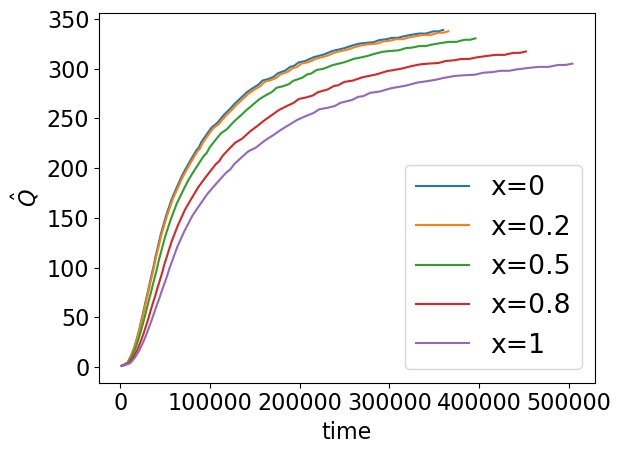
\includegraphics[width=0.6\textwidth]{fig/hydration_model_different_x_01_10_2022_17:13pdf.png}
    \caption{The available dataset $\mathcal{D} = \{\bm{\hat{x}}_{i},\bm{\hat{Q}}_{i}\}_{i=1}^{N}$ for the hydration model}
    \label{fig:hydration_datset}
\end{figure}

\begin{figure}[!htpb]
    \centering
    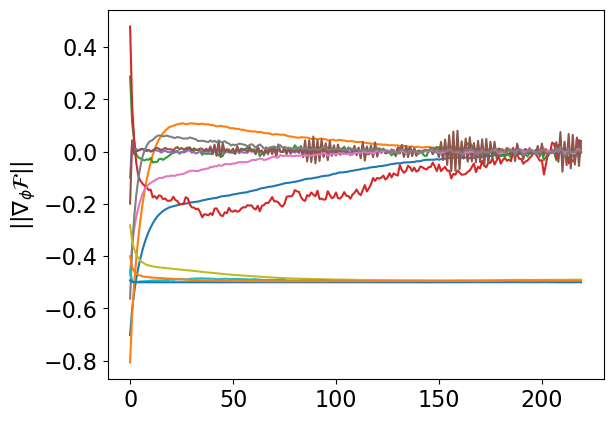
\includegraphics[width=0.6\textwidth]{fig/gradients_01_10_2022_17:13pdf.png}
    \caption{Evolution of the $ELBO$ gradeints w.r.t individual parameters $\varphi$.}
    \label{fig:ELBO_grad_evolution}
\end{figure}

\begin{figure}[!htpb]
    \centering
    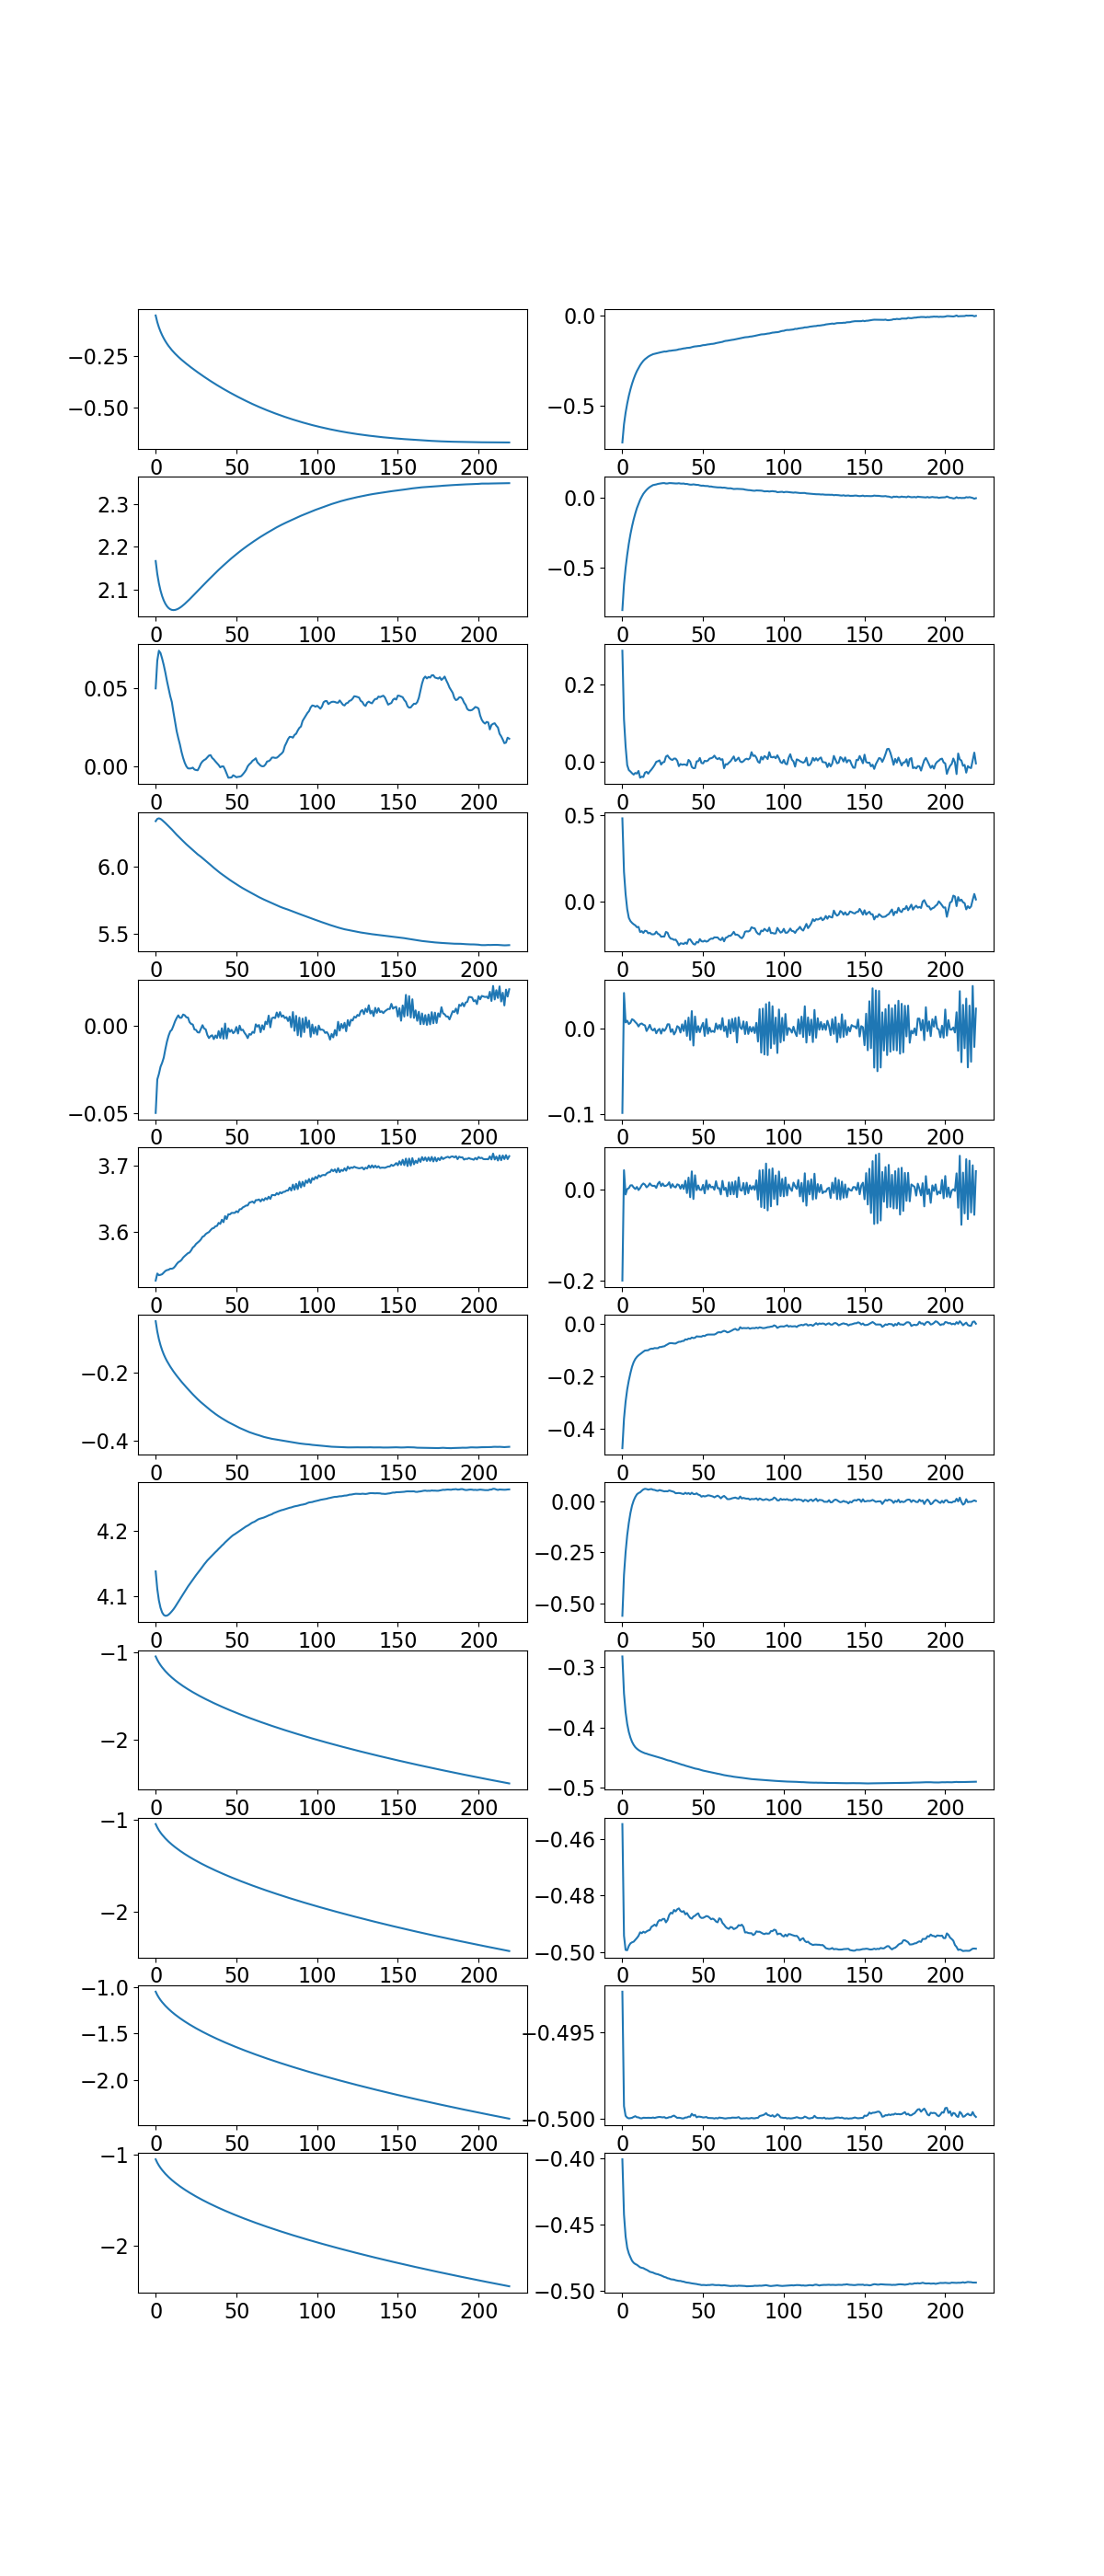
\includegraphics[width=0.6\textwidth]{fig/convergance_01_10_2022_17:13pdf.png}
    \caption{The evolution of parameters $\varphi$ and its gradients. The left column is parameter evolution and right the gradients}
    \label{fig:parameter_evolution}
\end{figure}

\begin{figure}[!htpb]
    \centering
    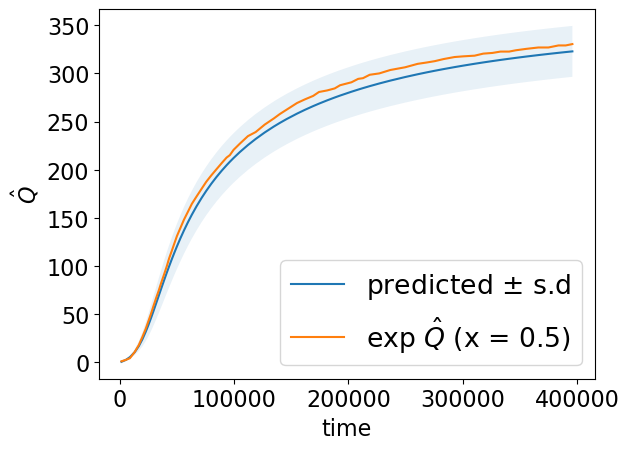
\includegraphics[width=0.6\textwidth]{fig/hydration_model_prediction_01_10_2022_17:13pdf.png}
    \caption{Evaluating the inferred parameters for the test dataset.The cem ratio $\bm x = 0.5$ is taken as test dataset. }
    \label{fig:hydration_model_prediction}
\end{figure}



\subsubsection{optimisation}

The task of optimization can be summarized as finding the optimum concrete mix parameters $\bm x$ (e.g, cement type ratio) to minimize certain (stochastic) objective such that some (stochastic) constraints are satisfied. Consider the following for the current formulation:

\begin{align}
	&\min_{\bm x} \E_{\bm b\sim p(\bm b | \bm x, \bm {\varphi}^*)}[y_{o_1}(\bm b)]\\
	&\text{s.t} ~~ \E_{\bm b\sim p(\bm b | \bm x, \bm {\varphi}^*)}[y_{o_i}(\bm b)] \leq \alpha_i, \quad i = 1,\cdots, m
\end{align}

Here, $\bm{\varphi}^*$ denotes the learnt parameters between the latents $\bm b$ and $\bm x$, $y_{o_1}$ denotes the solver output corresponding to the objective and $y_{o_i}$ the solver output corresponding to the $i^{th}$ constraint. Simplifying the notations a bit further, lets say $\mathcal{O}(\bm x)$ denotes the objective and $\mathcal{C}_{i}(\bm x)$ denotes the $i^{th}$ constraint. The problem can be approached with penalty based methods \footnote{\href{https://web.stanford.edu/class/ee364a/lectures/stoch_prog.pdf}{https://web.stanford.edu/class/ee364a/lectures/stoch_prog.pdf}}  as follows:

\begin{align}
	\min_{\bm x} \mathcal{O}(\bm x) + \sum_{i=1}^{m}c_i \mathcal{C}_i(\bm x)
\end{align}
where $c_i>0$ are penalty rates for violating constraints and the inequality constraint can be written as $\mathcal{C}_{i}(\bm x) = \max (\E_{\bm b\sim p(\bm b | \bm x, \bm {\varphi}^*)}[y_{o_i}(\bm b)] - \alpha_i,0)$. Alternatively, the problem can also  be approached with the Augmented Lagrangian Method \ref{appendix : Augmented Lagrangian}.

To test the scheme, a concrete column simulation with the hydration model is formulated \cite{} (@Erik can add the description if need be) for which the Key performance Indicator (KPI) is the critical time ($t_c$) at which the max yield is reached and there is a temperature constraint which says that the max. temperature ($T$) at no point in time should increase a certain value. Following the notations above, we have:

\begin{align}
&\min_{\bm x} \E_{\bm b\sim p(\bm b | \bm x, \bm {\varphi}^*)}[t_c(\bm b)]\\
&\text{s.t} ~~ \E_{\bm b\sim p(\bm b | \bm x, \bm {\varphi}^*)}[T(\bm b)] \leq \alpha
\end{align}

The problem is approached with penalty methods described above and score function gradient estimators (section.\ref{sec:optimisation_wo_constraints}) \cite{schulman_gradient_2016} are used to compute the expectation gradients. The implementation is performed in PyTorch library.
Some initial results are depicted in Fig. \ref{fig:opt_diagnostics_hydration} for $\alpha = 65^o$. As can be seen from the Fig. \ref{fig:para_opt_hydration}, the constraints started to be violated close to $\bm x \sim 0.6$ which led to negative gradients, which reversed the descend of the optimization parameter (by observation $t_c \propto 1/\bm{x}$) and stabilized it to a value which also satisfies the constraints.

\begin{figure}[!htpb]
	\centering
	\begin{subfigure}{0.45\textwidth}
		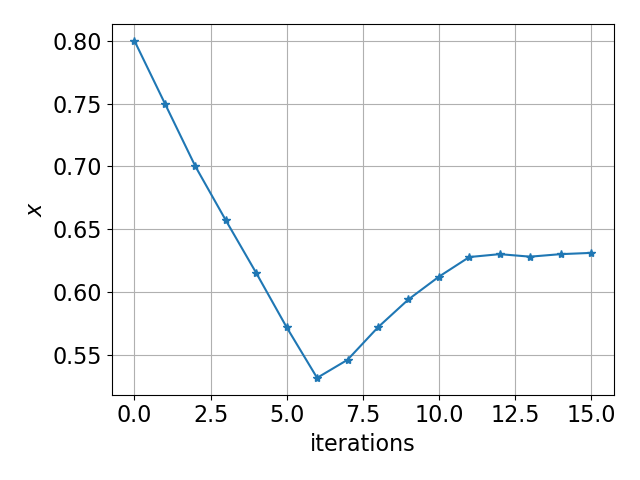
\includegraphics[width=\textwidth]{fig/x_evolution_stochastic_opt_wCOnstraints18_10_2022_13:06.png}
		\caption{Evolution of the optimisation variable $x$}
		\label{fig:para_opt_hydration}
	\end{subfigure}
	\hfill
	\begin{subfigure}{0.45\textwidth}
		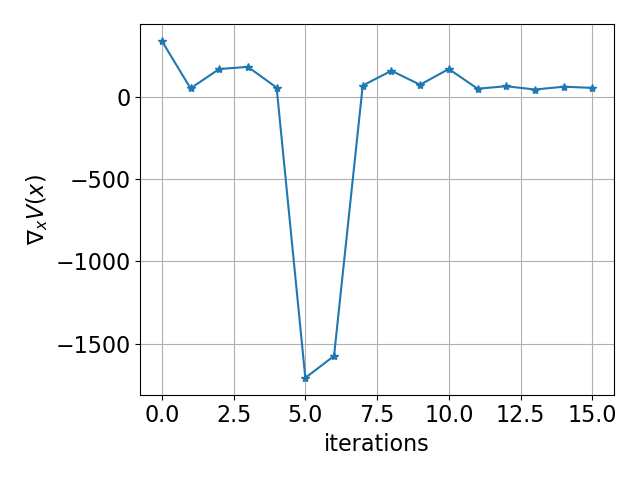
\includegraphics[width=\textwidth]{fig/grad_stochastic_opt_constraints18_10_2022_13:06.png}
		\caption{Monte Carlo estimated gradients}
		\label{fig:grad_opt_hydration}
	\end{subfigure}
	\hfill
	\caption{Optimisation under uncertainty for concrete column with hydration model}
	\label{fig:opt_diagnostics_hydration}
\end{figure}



 Its crucial to mention that computational cost of the forward solver can be a limiting factor in the optimization process. Efficient \textit{offline} surrogates can be developed for that. It can serve two purposes: i. Alleviate the computational bottleneck, ii. Potentially reduce the estimated variance of the gradients as reparametrisation trick can be used then (surrogate is differentiable). 

\clearpage
\appendix

\section{Stochastic Optimization with inequality constraints: The Augmented Lagrangian Method}\label{appendix : Augmented Lagrangian}
%\label{sec:stoptcon}
Consider the problem:
\be
\min_{\bs{x}} f(\bs{x}), \qquad \textrm{ such that $c(\bs{x})\le 0$ }
\ee
 We note that only noisy, Monte Carlo estimates of the aforementioned functions and their derivatives are available.
 One can define the Lagrangian:
 \be
 L(\bs{x},\lambda)=f(\bs{x})+\lambda c(\bs{x}), \qquad \lambda> 0
 \ee
 and perform the optimization:
 \be
 \min_{\bs{x}} \max_{\lambda > 0} L(\bs{x},\lambda)
 \ee
 One observes that if $c(\bs{x})\le 0$, then $\max_{\lambda>0} L(\bs{x},\lambda)=f(\bs{x})$ (for $\lambda=0$) and if $c(\bs{x})>0$, then $\max_{\lambda>0} L(\bs{x},\lambda)=+\infty$.
 The $\max_{\lambda}$ function is highly non-smooth w.r.t. $\bx$ and we smooth it by adding a regularization with respect to a distance to a proximal point. In particular if $\lambda^n$ is the estimate at iteration $n$ we define the {\em augmented}  Lagrangian (see \href{https://www.him.uni-bonn.de/fileadmin/him/Section6_HIM_v1.pdf}{here}).
%
\be
L^n(\bx,\lambda)=f(\bx) +\lambda c(\bx) -\frac{1}{2\rho} (\lambda-\lambda^n)^2
\ee
 This approach decomposes the constrained
problem into a sequence of unconstrained problems where Lagrange multipliers   are dynamically updated.
We note that:
\be
\frac{\pa L^n}{\pa \lambda}=0 \to \lambda^{n+1} =max(\lambda^n+\rho c(\bx),~0)
\label{eq:updatel}
\ee
and:
\be
\frac{\pa L^n}{\pa \bx}=\nabla f(\bx)+\lambda^{n+1} \nabla c(\bx)
\ee
Hence we propose iterating between:
\bi
\item updating $\bx$ using stochastic gradient descent and Monte Carlo estimates of $\frac{\pa L^n}{\pa \bx}$ above.
\item updating $\lambda$ as in \refeq{eq:updatel} where $\rho$  is a fixed step-size (regularization term). This involves a Monte Carlo estimate of the constraint $c(\bx)$.
\ei

% adding Bib
\newpage
\nocite{*}
\bibliographystyle{unsrt}
%\bibliographystyle{abbrv}
\footnotesize{\bibliography{bibliography.bib}}
\end{document}


